\documentclass[tikz, border=5pt]{standalone}
\usetikzlibrary{perspective, arrows.meta}

\begin{document}

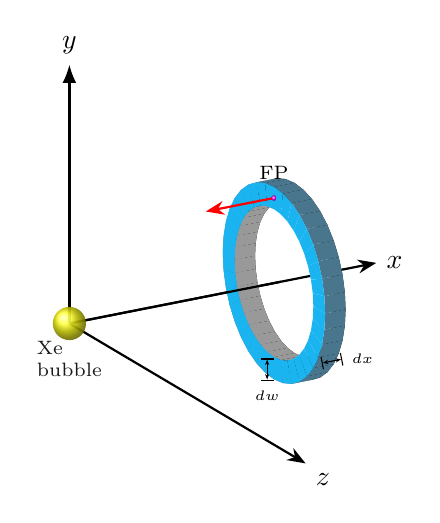
\begin{tikzpicture}[3d view={60}{20}, >=Stealth]
	% relabel xyz at the very end
	\draw[->, thick] (0, 0, 0) -- (6.0, 0, 0) node[below right] {$z$};
	\draw[->, thick] (0, 0, 0) -- (0, 4.5, 0) node[right] {$x$};
	\draw[->, >=Latex, thick] (0, 0, 0) -- (0, 0, 3.5) node[above] {$y$};

	\def\r{1.0}
	\def\R{1.3}
	\def\h{3.0}
	\def\H{3.3}

	% outer
	\foreach \x in {0, 10, ..., 350} {
		\fill[black]
			({\r*cos(\x)},    \H, {\r*sin(\x)}) --
			({\R*cos(\x)},    \H, {\R*sin(\x)}) --
			({\R*cos(\x+10)}, \H, {\R*sin(\x+10)}) --
			({\r*cos(\x+10)}, \H, {\r*sin(\x+10)}) -- cycle;
	}

	% upper
	\foreach \x in {0, 10, ..., 350} {
		\fill[cyan!50!black]
			({\R*cos(\x)},    \h, {\R*sin(\x)}) --
			({\R*cos(\x)},    \H, {\R*sin(\x)}) --
			({\R*cos(\x+10)}, \H, {\R*sin(\x+10)}) --
			({\R*cos(\x+10)}, \h, {\R*sin(\x+10)}) -- cycle;
	}

	% lower
	\foreach \x in {90, 100, ..., 290} {
		\fill[gray!80]
			({\r*cos(\x)},    \h, {\r*sin(\x)}) --
			({\r*cos(\x)},    \H, {\r*sin(\x)}) --
			({\r*cos(\x+10)}, \H, {\r*sin(\x+10)}) --
			({\r*cos(\x+10)}, \h, {\r*sin(\x+10)}) -- cycle;
	}

	% inner
	\foreach \x in {0, 10, ..., 350} {
		\fill[cyan!90]
			({\r*cos(\x)},    \h, {\r*sin(\x)}) --
			({\R*cos(\x)},    \h, {\R*sin(\x)}) --
			({\R*cos(\x+10)}, \h, {\R*sin(\x+10)}) --
			({\r*cos(\x+10)}, \h, {\r*sin(\x+10)}) -- cycle;
	}

	\draw[->, red, thick]
		(0, \h, {(\r+\R)/2}) -- +(0, -1, 0);
	\shade[ball color=magenta]
		(0, \h, {(\r+\R)/2}) circle [radius=1pt]
		node [above=3pt, font=\scriptsize] {FP};

	% fixing the axis
	\draw[thick] (0, 0, 0) -- (0, 3.1, 0);

	\begin{scope}[>={Stealth[length=2pt]}]
		\draw[|<->|]
			({(\R+0.1)*cos(-30)}, \h, {(\R+0.1)*sin(-30)}) --
			({(\R+0.1)*cos(-30)}, \H, {(\R+0.1)*sin(-30)})
			node [right, font=\tiny] {$dx$};

		\draw[|<->|]
			({\r*cos(-90)}, \h-0.1, {\r*sin(-90)}) --
			({\R*cos(-90)}, \h-0.1, {\R*sin(-90)})
			node [below, font=\tiny] {$dw$};
	\end{scope}


	\shade[ball color=yellow, opacity=0.9]
		(0, 0, 0) circle [radius=6pt]
		node [below=3pt, font=\scriptsize, align=left] {Xe\\bubble};

\end{tikzpicture}

\end{document}
